\chapter{Client-Side JS: Browser APIs}
\label{browser-apis}
\paragraph{} JavaScript is how we add dynamism to our web pages mostly through a set of global JS objects which provide access to the client environment. So now we have a working knowledge of Javascript, we'll start to look at how it can be used to manipulate the HTML that makes up our webpages, as well as to interact with the browser. If we think of the browser as the host environment that defines the space in which our Javascript functions run, then it is useful to explore what features of the environment are made available to us through the Browser's Application Programming Interfaces (Browser’s APIs).


\section{JS \& HTML}
\paragraph{} In the last unit we considered how JS practically interacts with other web technologies. In particular:

\begin{itemize}
\item JS isn’t self-hosted within the browser. That is we can't just retrieve a JS file directly from a web address and run it. The JS has to be hosted within a page. A minimal host document is required to cause the browser to then retrieve our JS. Once retrieved the JS is then loaded and executed by the browser's JS engine.
\item JS can be:
    \begin{itemize}
    \item added inline with HTML elements, 
    \item spread throughout our document, or 
    \item added as a block collected into a single place within a document, or as an external/linked file(s)
    \end{itemize}
\end{itemize}

\paragraph{} Note that our examples from the last unit were all run in the browser web console. Whilst strictly speaking this means we can run JS in the browser, it actually gives us a fairly rich environment for executing JS, learning the language, and experimenting, but it isn't generally how we would distribute our JS code to end-users

\paragraph{} We’ll investigate this a little more and use it as a motivating framework for exploring interactions between HTML and JS. In the last unit we briefly surveyed three methods by which JS can be integrated with HTML. Let's recap those now.


\section{Recap: A Simple Inline JS Example}
\paragraph{} In this example we have our JS entirely encapsulated within the onclick function of an HTML button element.

\begin{lstlisting}
<!DOCTYPE html>
<html>
  <head>
    <title>Example</title>
  </head>
  <body>
      <button onclick="var textNode = document.createTextNode(‘Napier!');
 			document.body.appendChild(textNode);">Hello</button>
  </body>
</html>
\end{lstlisting}

\paragraph{} This means that our JS is localised entirely to the specific button element that it is attached to and can't be reused elsewhere, for example, if we have similar code attached to another button. This means that you need to repeat code across your pages, as well as mix JS amongst your HTML. Generally this is a bit of a "code smell" and, whilst useful for quickly trying out some code, is not an ideal solution.


\section{Recap: A Simple JS Script Block Example}
\paragraph{} This version moves our JS into its own script block. Note that it doesn't do anything more than our last, inline, version. In fact it needs a little bit more code to achieve the same effect. This is mainly because the inline version is immediately attached to its HTML element and the context in which it runs. Now we've separated our JS from the HTML element it affects, we have to add additional code to get a 'handle' on the original HTML element. In this case we've achieved our aims by adding an ID to the button and then using getElementById to create the link between our JS and the button element.

\begin{lstlisting}
<!DOCTYPE html>
<html>
  <head>
    <title>Example</title>
  </head>
  <body>
    <button id="hello_btn">Hello</button>
    <script>
        document.getElementById('hello_btn').onclick = function() {
           var text_node = document.createTextNode('Napier!');
            document.body.appendChild(text_node);   
        };
    </script>
  </body>
</html>
\end{lstlisting}

\paragraph{} Overall, the JS is now reasonably separated from the HTML elements within the page which means that functions can be more easily organised and reused in multiple places. Whilst the JS is still hosted within the parent HTML document it is encapsulated within a pair of script tags. This actually makes it much easier to move to the next integration method\dots


\section{Recap: A Simple JS Eternal Script Example}
\paragraph{} In this example our JS is now entirely stored within a separate file. First our index.html file:

\begin{lstlisting}
<!DOCTYPE html>
<html>
  <head>
    <title>Example</title>
  </head>
  <body>
    <button id="hello_btn">Hello</button>
    <script src="tmp.js"></script>
  </body>
</html>
\end{lstlisting}

\paragraph{} and then our index.js file:

\begin{lstlisting}
document.getElementById('hello_btn').onclick = function() {
    var text_node = document.createTextNode('Napier!');
        document.body.appendChild(text_node);   
};
\end{lstlisting}

\paragraph{} Notice that we still have a script tag in the HTML file, but it now just points to a web address where the JS is located and can be retrieved from. Again, the only link between the HTML element, our button, and the JS that is executed when the button is pressed is the button's ID.
\paragraph{} The pattern found in this example is probably the most standard framework for relating JS and HTML, keeping a useful separation of concerns that can lead to better manageability and increased reusability of code.



\section{A Slightly More Complex Example}
\paragraph{} The last example was fairly static though, it didn't do much other than wait for user input. The following example goes a little further. As well as giving us a button that, when clicked, adds text to the page, we're also actually building the page itself. Look at the body of our HTML file. It doesn't actually contain any HTML elements, so where is our interface coming from? It turns out that we're building it entirely through JS code! This is a really powerful opportunity that JS provides us for dynamically changing the pages that our users see.

\begin{lstlisting}
<!DOCTYPE html>
<html>
  <head>
    <script src="tmp.js"></script>
  </head>
  <body>
  </body>
</html>
\end{lstlisting}

\paragraph{} and our index.js file:

\begin{lstlisting}
function init() {
    document.title = "Hello Napier Example"

    var button = document.createElement("button");
    button.innerHTML = "Hello";
    button.id = "hello_btn";
    var body = document.getElementsByTagName("body")[0];
    body.appendChild(button);

    document.getElementById('hello_btn').onclick = function() {
        var text_node = document.createTextNode('Napier!');
            document.body.appendChild(text_node);   
    };
};
window.onload=init;
\end{lstlisting}


\section{The JS-HTML Relationship}
\paragraph{} On a practical level the JS-HTML relationship, where an HTML document references some JS that then runs, is a simplified way of looking at things. It is actually not merely the case that the browser retrieves an HTML document, which in turn references some JS, which then just runs.
\paragraph{} The reality is a little more complex. You can get away with the above understanding but you’ll miss a lot of powerful functionality if you don’t consider the wider context of the DOM (the Document Object Model) and the browser environment. A lot of rich possibilities are created by the set of APIs that the DOM and browser environment provide.
\paragraph{} To understand this relationship, and to start seeing some of the possibilities that are provided, we’re going to primarily consider the following in this unit:

\begin{itemize}
\item The Window Object
\item The Document Object
\end{itemize}



\section{The Window Object Hierarchy}
\paragraph{} The Window object is the root of a tree of browser and web page related objects along with their associated APIs. One of the children of the Window object is the document object, which gives us access to the DOM. All of the other children give us access to the wider infrastructure that we can manipulate, all related to the browser window. Not only are we able to interact with the parsed HTML document (our current page) but also with a wide range of additional related aspects of the browser. 
\paragraph{} More specifically these are additional objects that JS can access and hence we can write JS code to manipulate them within the boundaries provided by their respective APIs.
\paragraph{} Note that there are browser differences which mean that some objects are available on some platforms/versions and not on others. For the most part this is not an issue, but you should be aware of the possibility. The diagram gives you an idea of the range of objects that are accessible to our JS code.

\begin{figure}[H]
\centering
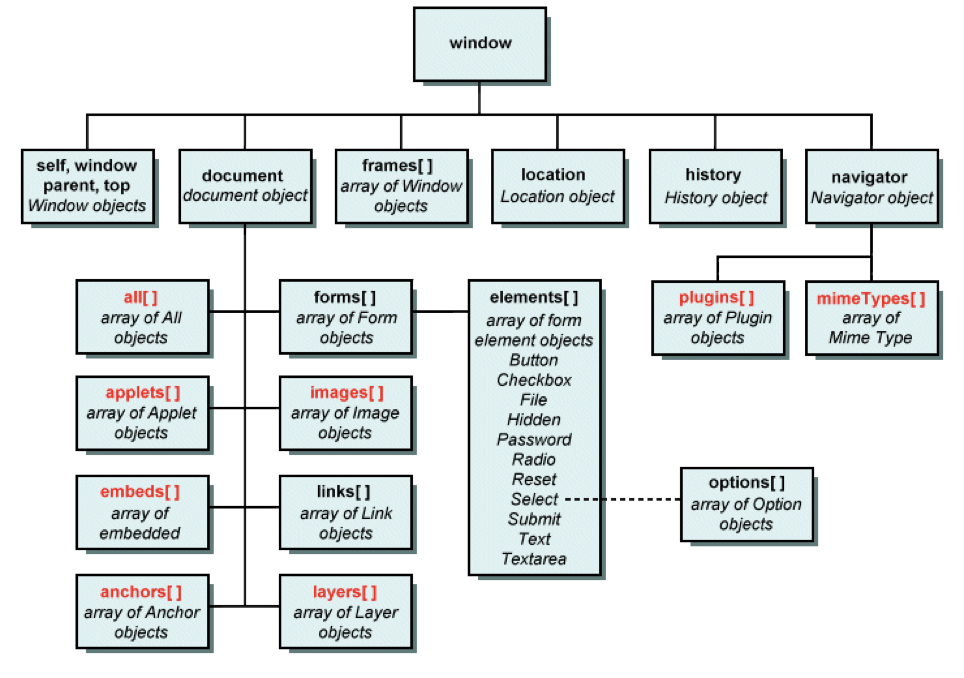
\includegraphics[width=0.8\textwidth]{figures/window-object-hierarchy}
\label{fig:window-object-hierarchy}
\caption{}
\end{figure}



\section{Global Objects}
\paragraph{} First an aside about global objects and scope. Generally our JS code is either associated with a Window and hence has a Window object associated with it, or else it runs in a separate background task within the browser. We'll not specifically cover background tasks here, they are a way to run your code "in the background" so that it doesn't interfere with the responsiveness of the current tab. This can be very useful for more involved JS applications so if you want to know more then it is worth researching the term "webworkers" if you do want to run bits of code independently in the background.
\paragraph{} The window object is a global object. This means that it is always in scope or has “global scope”. Any JS variables that you create outside a function also have global scope. Additionally any JS functions that you create outside an object have global scope. What does this mean? That we can always access the Window object, from any part of our code, and that any global variables, or functions that we create are also accessible via the Window object. If we define a global JS variable or function then we can always access it via the window object as a property of the global object.
\paragraph{} Let's look at an example of that:

\begin{lstlisting}
var daka = “more daka”;
daka === window.daka;
// This will evaluate to true if the daka variable is available via the window object

function hi() {console.log(“hi”);}
window.hi === hi;
// Will evaluate to true for the same reasons as above
\end{lstlisting}

\paragraph{} All we've done in the example is to create a variable and a function with global scope, then demonstrated that they are accessible through the Window object.


\section{The Window Object}
\paragraph{} The Window object represents an open browser window, or a tab within a window, for browsers which support tabs. The Window object contains a document object, representing the DOM, the parsed and instantiated set of objects that the browser creates to represent the HTML element described in the source HTML document.
\paragraph{} So our HTML page, as identified by the Web address we've navigated to, is a part of the Window object via the document/DOM child object, but it also gives access to much more.
\paragraph{} For example, a single window could use HTML frames to display multiple HTML pages in the same window, so there is also support for listing, retrieving, and interacting with frames and hence the pages they contain, using the window.frames property.
\paragraph{} Similarly we can find out information about the browser that our page is loaded into via the window.navigator property. This can be used to retrieve, for example, the name of the browser application and its version.
\paragraph{} We can also interact with the history of the current window. By history we mean the list of pages that have been navigated since the current window/tab was opened. Each time you successfully navigate a hypertext link the new page is displayed and the last page is added to the history list. We can find out how long the list of previous pages is and we can use JS to navigate backwards and forward sequentially or to jump backwards and forward between pages. We can also interact with the location (URL/address) of the current page using the window.location property.


\section{The Console Object because ``There will be bugs''}
\paragraph{} The console object provides a really useful set of functions for debugging activities. When you write code, such as JS, you will create bugs. As your code becomes more elaborate, then you are more likely to accidentally introduce bugs. Whilst you will get better at noticing bugs related to syntax, for example, mis-spelling a keyword you will eventually start to create much more subtle bugs, the kind that don't cause a catastrophic crash but are more subtle and corrupt your data or give rise to incorrect results. These bugs are much more difficult to solve. In addition to using the debugging tools that are amongst most  modern desktop browser's suite of developer tools, you can also use the Console object from within your JS code to create log messages of information from within your program. These log messages are displayed in the browser console, and can also be searched and filtered using the browser console tools.
\paragraph{} The console logging functions include console.log, console.info, console.warn, and console.error and can be used to segregate output that is merely informational from output that is important and giving details about errors. You as a developer must decide how important the output is and decide which style of console logging to use for each message that you want to log.
\paragraph{} Logging works by passing a message, a string, to the function, e.g.

\begin{lstlisting}
console.log("Hello Napier");
\end{lstlisting}

\paragraph{} You can also pass CSS styles to logging functions, e.g.

\begin{lstlisting}
console.log("%c hello", "background: #222; color: #bada55");
\end{lstlisting}

\paragraph{} This can make the console much more easy to navigate so that you can find debug information when needed.

\paragraph{} The console also provides access to several other useful debug features that are useful when developing and evaluating our code. These include timing functions, counting and grouping functions, as well as standard debug features like assert() and trace(). We'll look at examples of each over the next few sub-sections.



\subsection{Console Timer Example}
\paragraph{} Sometimes we want to know when something happened, or how long something took to complete, so we use the console.time function to find out. In the following code we create a timer instance, ``t1'' then send log messages to that timer instance before finally ending the timer when we're done. Each call to timelog and timeEnd causes the elapsed time to be displayed in the console.

\begin{lstlisting}
console.time('t1');
console.timeLog('t1', 'starting engines...');
console.timeLog('t1', 'in ur code, doing your things...');
console.timeLog('t1', "work complete, shutting down...");
console.timeEnd('t1');
\end{lstlisting}



\subsection{Console Count() Example}
\paragraph{} Rather than how long something took, sometimes we just want to know how many times something occurred. This ability is what the count function gives us. In the following example we are using the count function to count how many times the greet function is called.

\begin{lstlisting}
let user = "";

function greet() {
  console.count();
  return "hi " + user;
}

user = "bob";
console.log(greet());
user = "alice";
console.log(greet());
console.log(greet());
\end{lstlisting}

\paragraph{} We can also give our counter a label, e.g."alice" so that it can be distinguished from the "default" counter like so:

\begin{lstlisting}
console.count("alice");
\end{lstlisting}



\subsection{Console Group() Example}
\paragraph{} Because our JS programs might become quite large and complex, it can be useful to group and organise our log messages. The console.group function enables us to do this. The console.group function hierarchically groups debug and log output together to make it easier to navigate in the console. Let's look at an example:

\begin{lstlisting}
console.log("This is the outer level");
console.group();
console.log("Level 2");
console.group();
console.log("Level 3");
console.warn("More of level 3");
console.groupEnd();
console.log("Back to level 2");
console.groupEnd();
console.log("Back to the outer level");
\end{lstlisting}

\paragraph{} Running this code in the browser console will give output similar to this:

\begin{figure}[H]
\centering
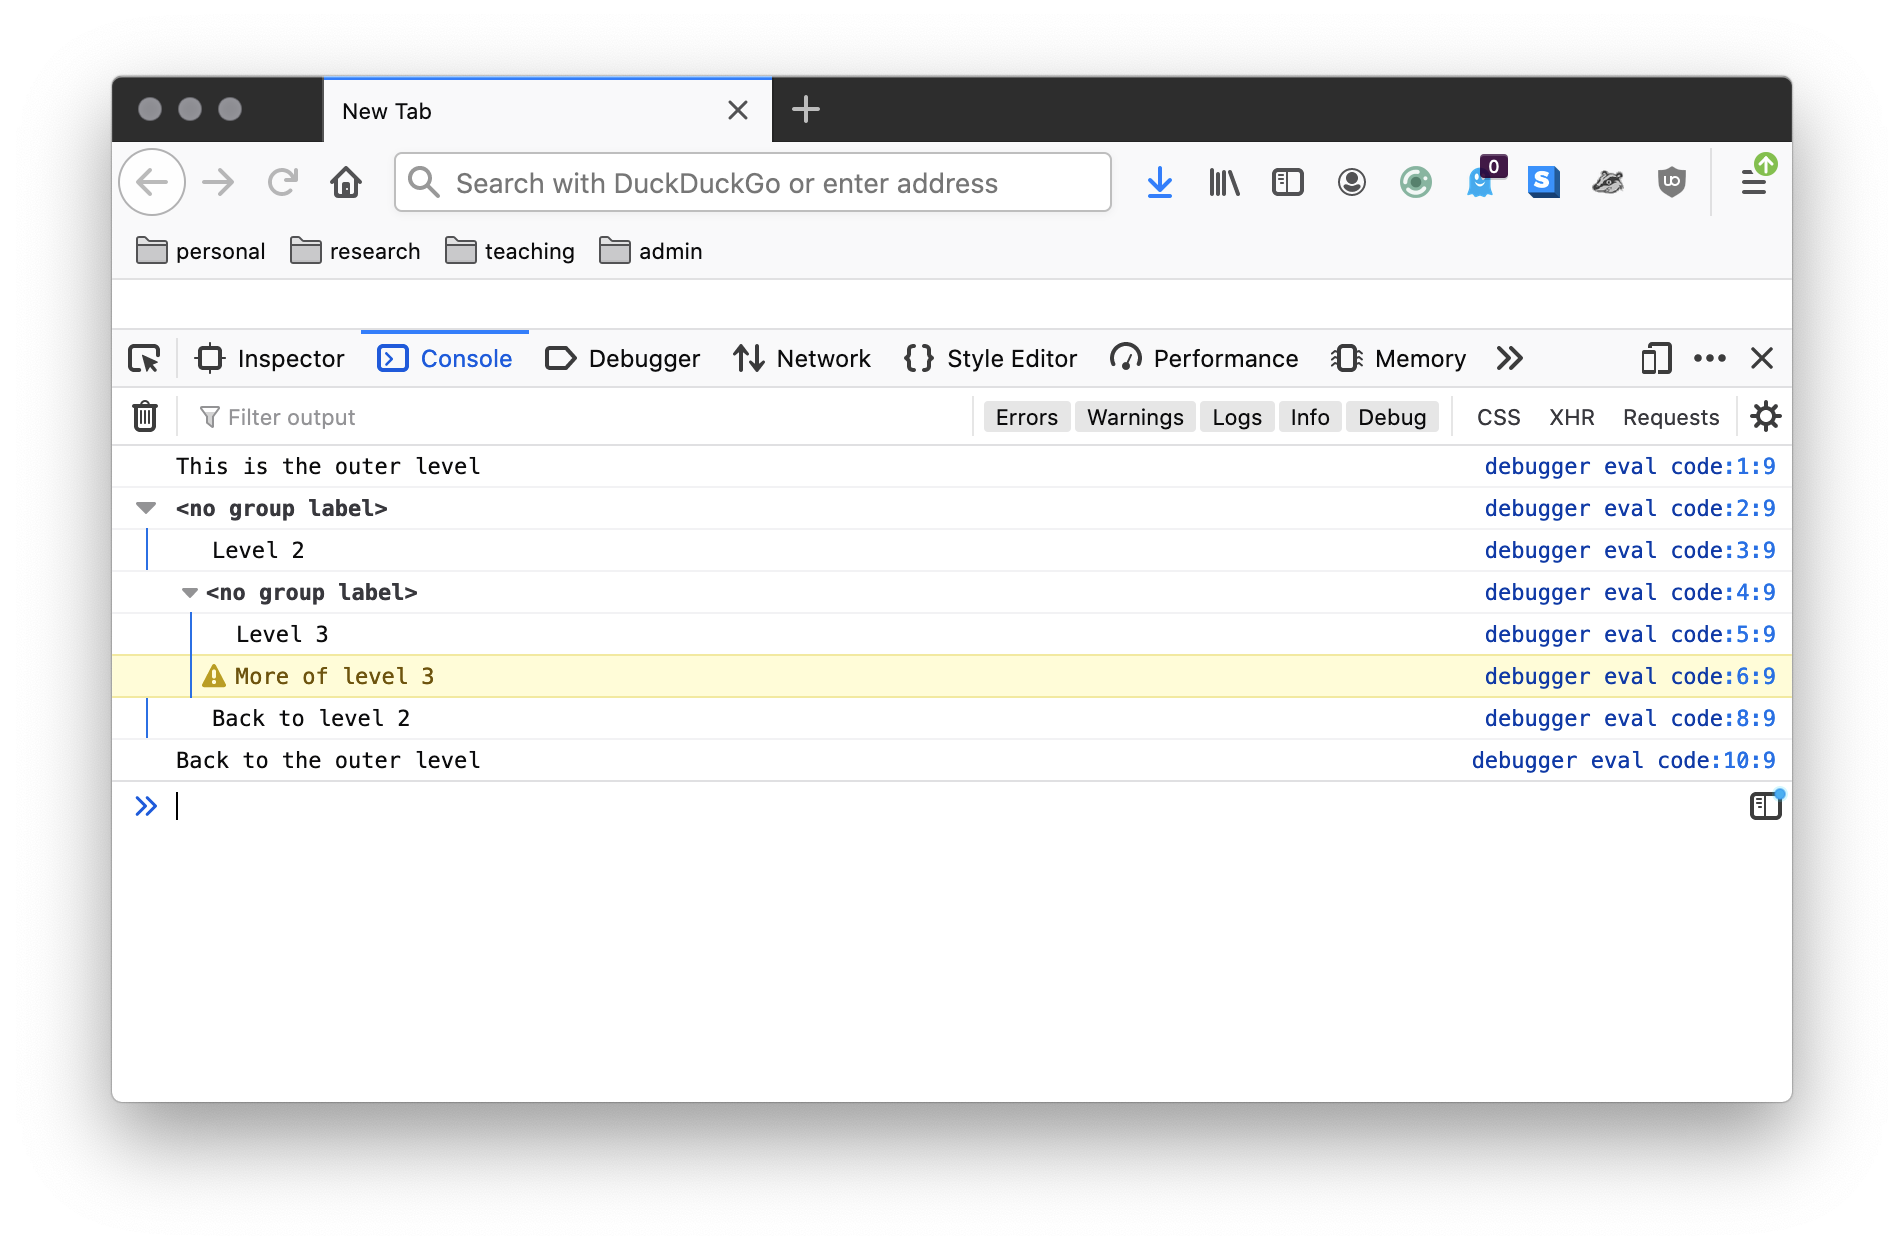
\includegraphics[width=0.8\textwidth]{figures/console-group}
\label{fig:console-group}
\caption{}
\end{figure}



\subsection{Console Assert Example}
\paragraph{} Assertions are used in many programming languages as a way to verify that our expectations about the way that a piece of code works actually match the reality of how it works. The basic idea is that we make an assertion, i.e. the value of variable x at this point in the program is y, and then the actual values of x and y are compared to each other and the assertion is true if they match and false otherwise. Let's look at a small example:

\begin{lstlisting}
const errorMsg = 'the # is not even';
for (let number = 2; number <= 5; number += 1) {
    console.log('the # is ' + number);
    console.assert(number % 2 === 0, {number: number, errorMsg: errorMsg});
}
\end{lstlisting}

\paragraph{} Running this code in the browser console will give output similar to this:

\begin{figure}[H]
\centering
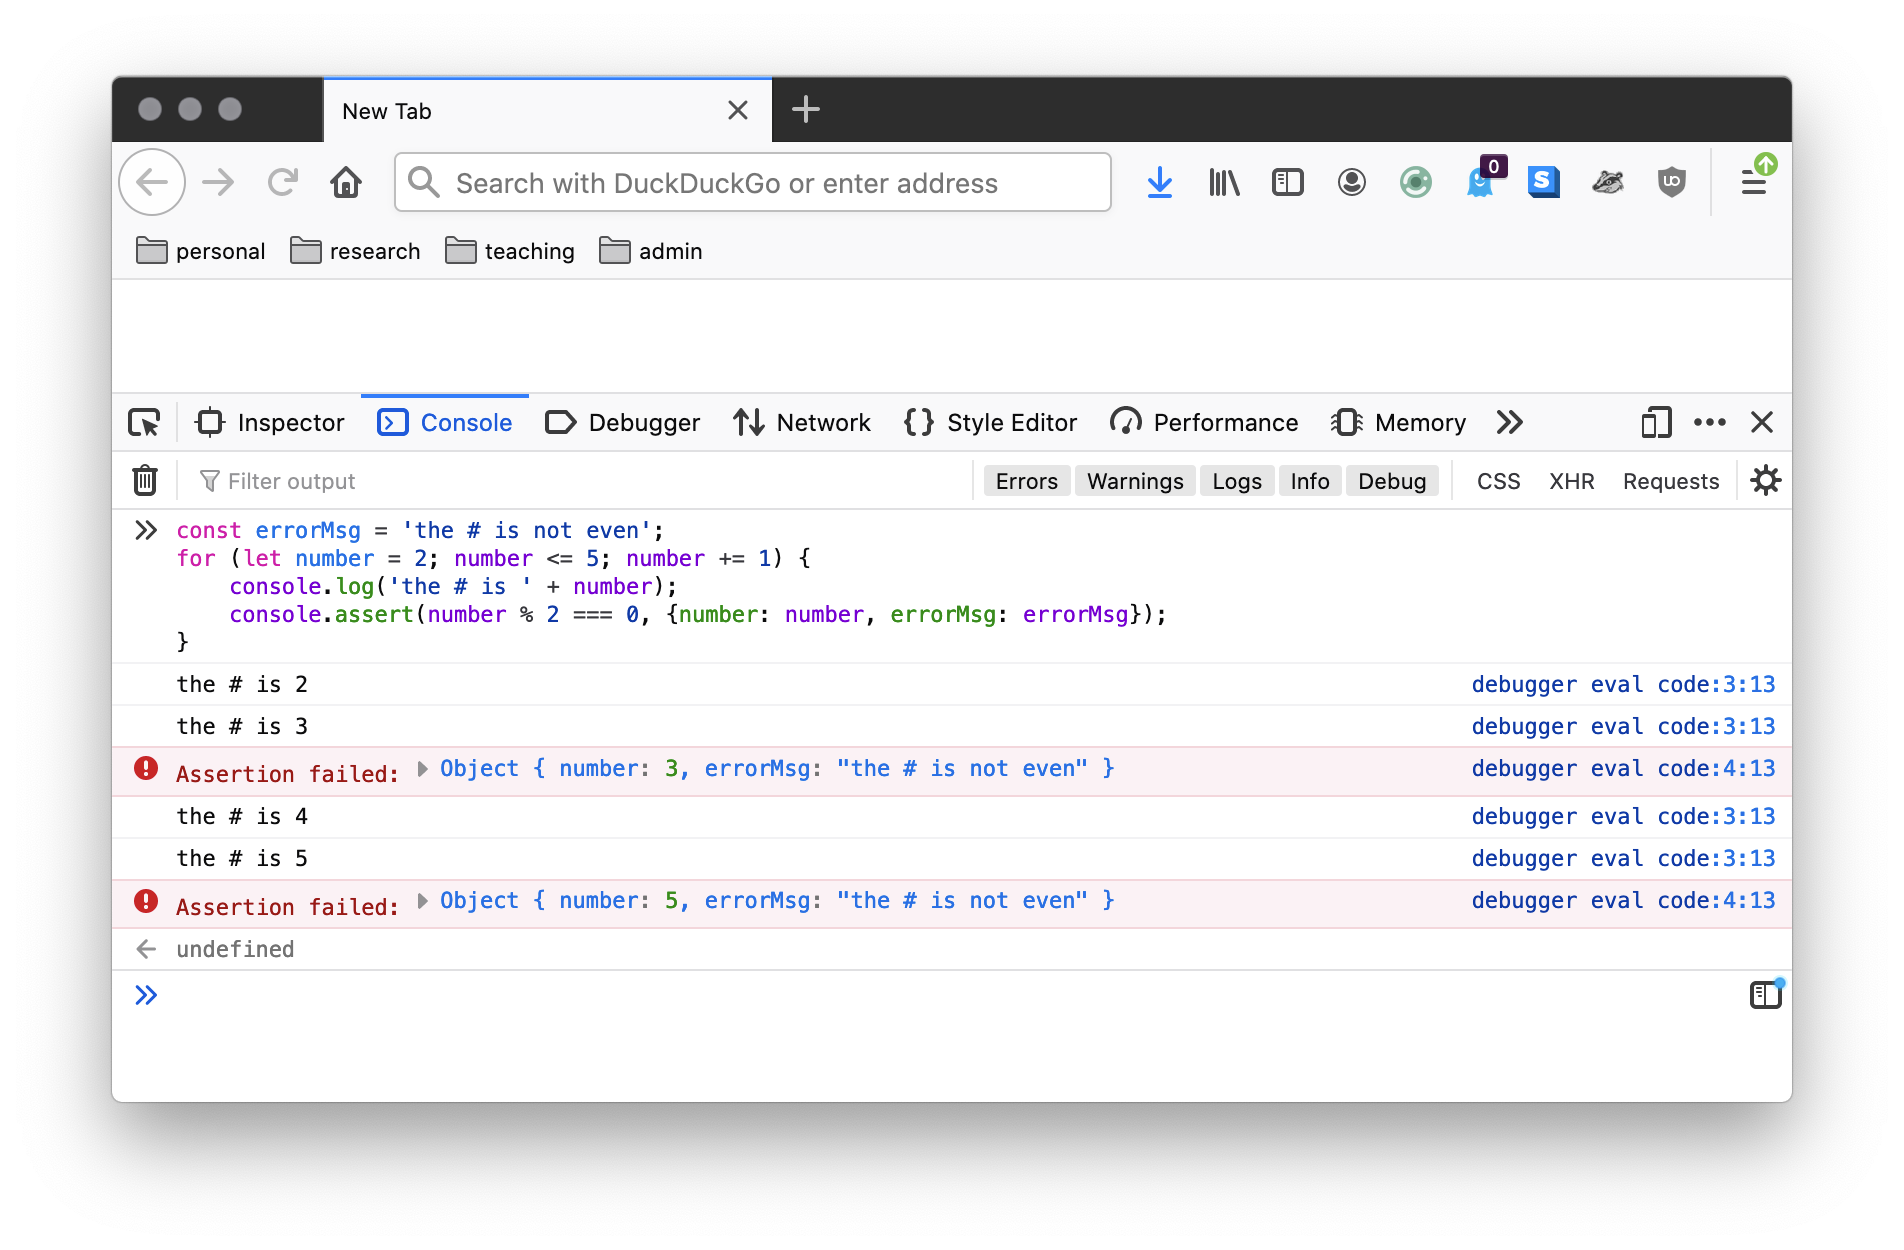
\includegraphics[width=0.8\textwidth]{figures/console-assert}
\label{fig:console-assert}
\caption{}
\end{figure}


\subsection{Console Trace Example}
\paragraph{} Sometimes we want to trace the stack of function calls that have led to the current situation in our running JS code. The console.trace function lets us do this.

\begin{lstlisting}
function foo() {
  function bar() {
    console.trace();
  }
  bar();
}

foo();
\end{lstlisting}

\paragraph{} Running this code in the browser console will give output similar to this:

\begin{figure}[H]
\centering
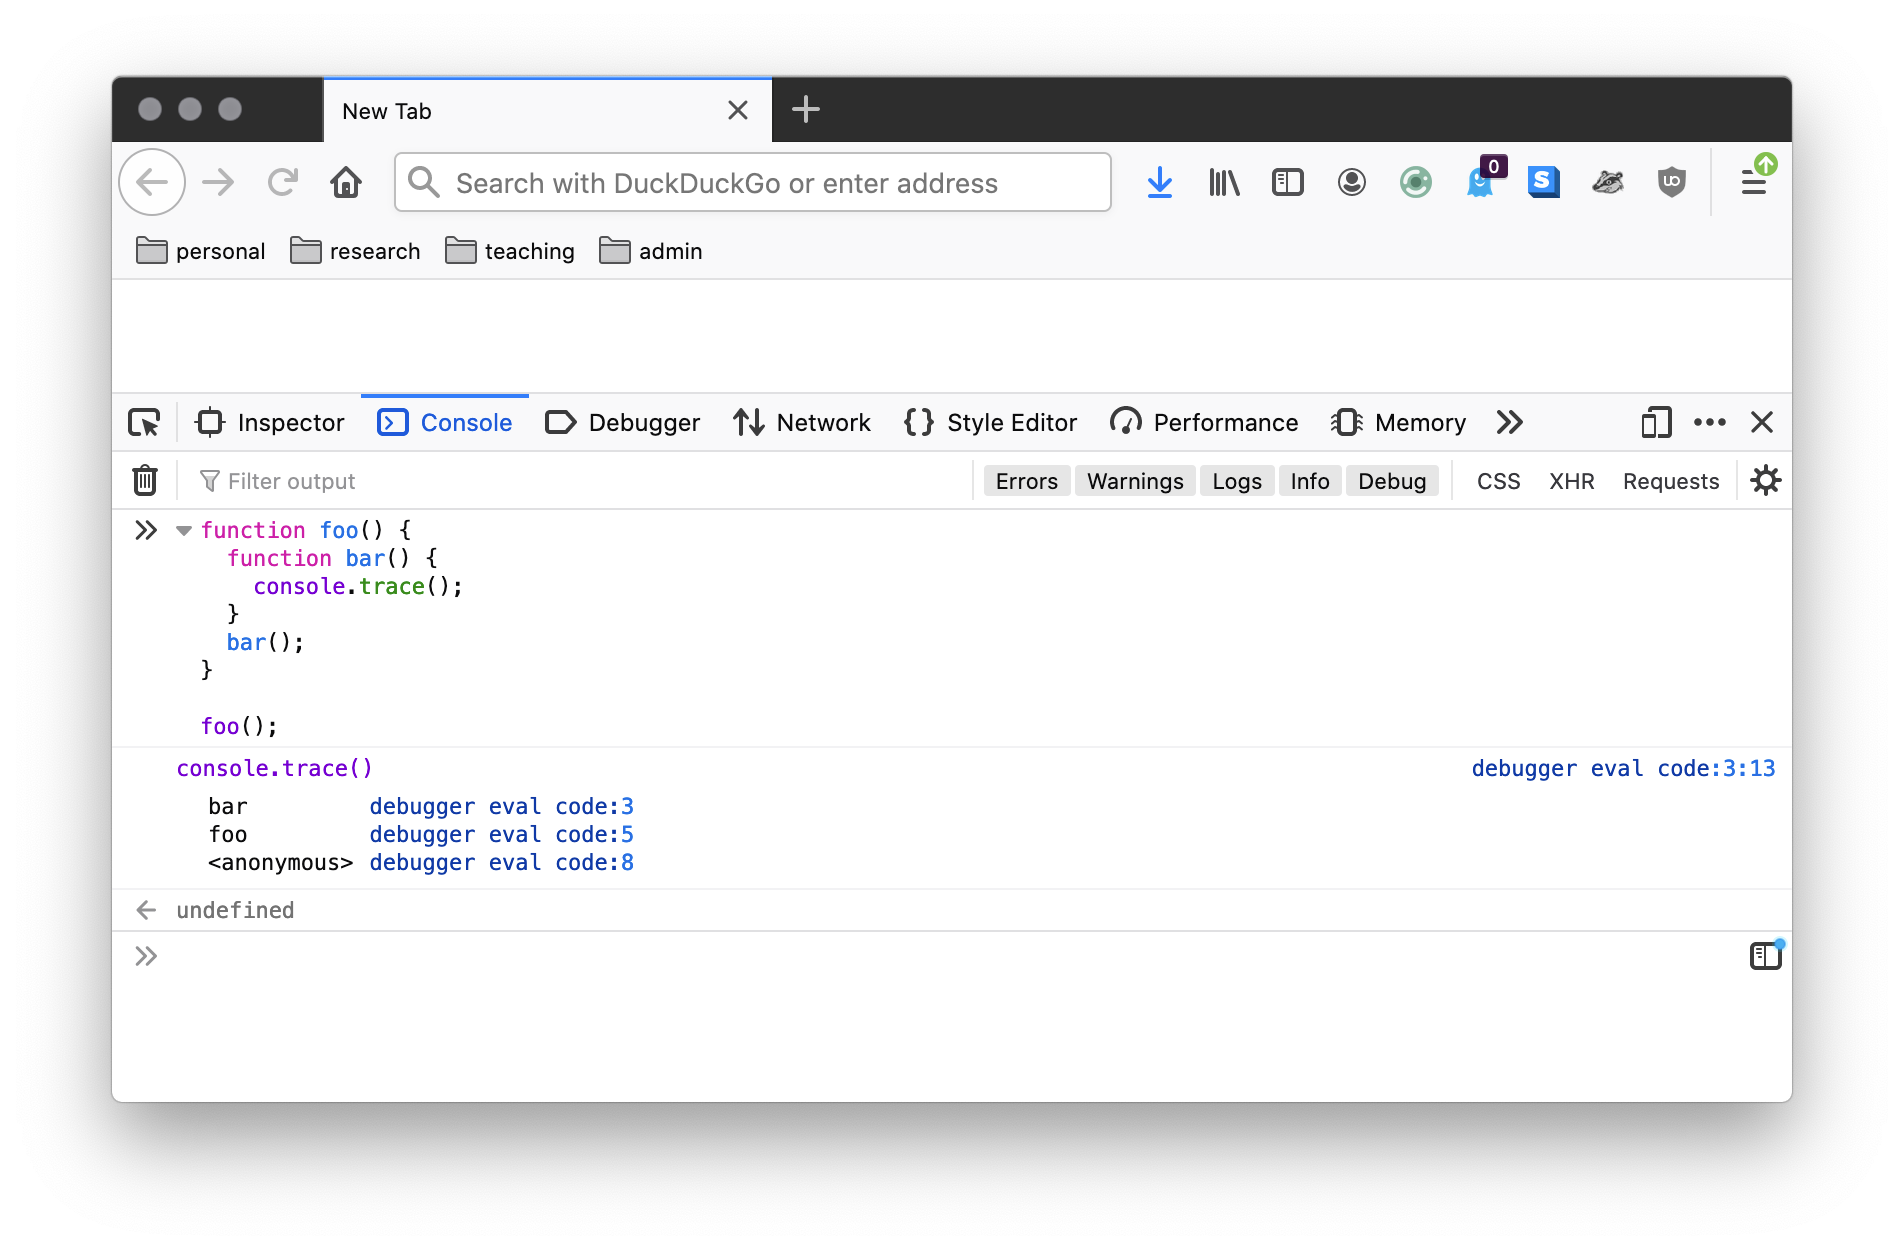
\includegraphics[width=0.8\textwidth]{figures/console-trace}
\label{fig:console-trace}
\caption{}
\end{figure}


\section{History Object}
\paragraph{} Returning to the Window object again, let's examine the History object. This stores the list of URLs that the user has visited within the current browser window or tab. It doesn't give access to other tabs however, only the current one. Access to specific URLs that might previously have been visited is prohibited, as is access to other windows or tabs that the browser might have opened. This is for both security and privacy reasons and aims to keep individual windows and tabs relatively isolated from each other.

\paragraph{} The History Object has the following properties:

\begin{itemize}
\item length -  the number of URLs in the history list
\end{itemize}

\paragraph{} The following methods are also available for use:

\begin{itemize}
\item back() -  Load the previous URL
\item forward() - Load the next URL
\item go() - Load a specific URL from the list by jumping n places (positive or negative) to move that amount through the history list
\end{itemize}

\paragraph{} Note that the history object is not standardised but is supported in the above format by major browsers, so you might find some more esoteric browsers whose behaviours differ.


\section{Navigator Object}

\paragraph{} The Navigator object stores information about the browser. The properties that are available and which can be retrieved include the following list (which is not exhaustive):

\begin{itemize}
\item appName - Returns the browser name
\item appVersion - Returns the version of the browser
\item cookieEnabled - Are cookies enabled?
\item platform - Which OS is this browser installed on?
\item userAgent - Access the header sent by the browser to the server to self identify
\end{itemize}

\paragraph{} Note that again, the navigator object is not standardised but is supported in the above format by most major browsers.


\section{Screen Object}
\paragraph{} Similar to the Navigator object, the screen object is a source of information about the screen that the user’s browser is displayed on. This can be useful, for example, when using different layouts and trying to decide when to switch from one to another.

\paragraph{} The supported properties include:

\begin{itemize}
\item availHeight - Height of screen minus certain furniture, e.g. windows taskbar
\item availWidth - Width of screen minus certain furniture, e.g. windows taskbar
\item height - Total height of the screen
\item pixelDepth - Colour resolution in bits per pixel
\item width - Total width of the screen
\end{itemize}

\paragraph{} Note that, as for the Navigator and History objects, the Screen object is not standardised but is supported in the above format by major browsers (do you notice a theme developing here\ldots?).


\section{Document Object Model}
\paragraph{} Now, having surveyed all of the other child objects of the Window object, let's turn our attention to the Document object and the Document Object Model (DOM). When an HTML file is retrieved and loaded the HTML tags are parsed into a hierarchical data structure, a tree, that more-or-less matches the structure of our HTML. The key difference is that this data structure, the DOM, is easier to manipulate, i.e. from JS code (or CSS). The browser uses the DOM during the rendering process and is a critical underpinning metaphor or model for the way that most modern browsers operate. Once an HTML file is parsed, the browser ignores it and prefers to use only its internal DOM representation of the page. Here is a basic illustration of a simple HTML document parsed into a DOM representation. Obviously things can become much more complex than this.


\begin{figure}[H]
\centering
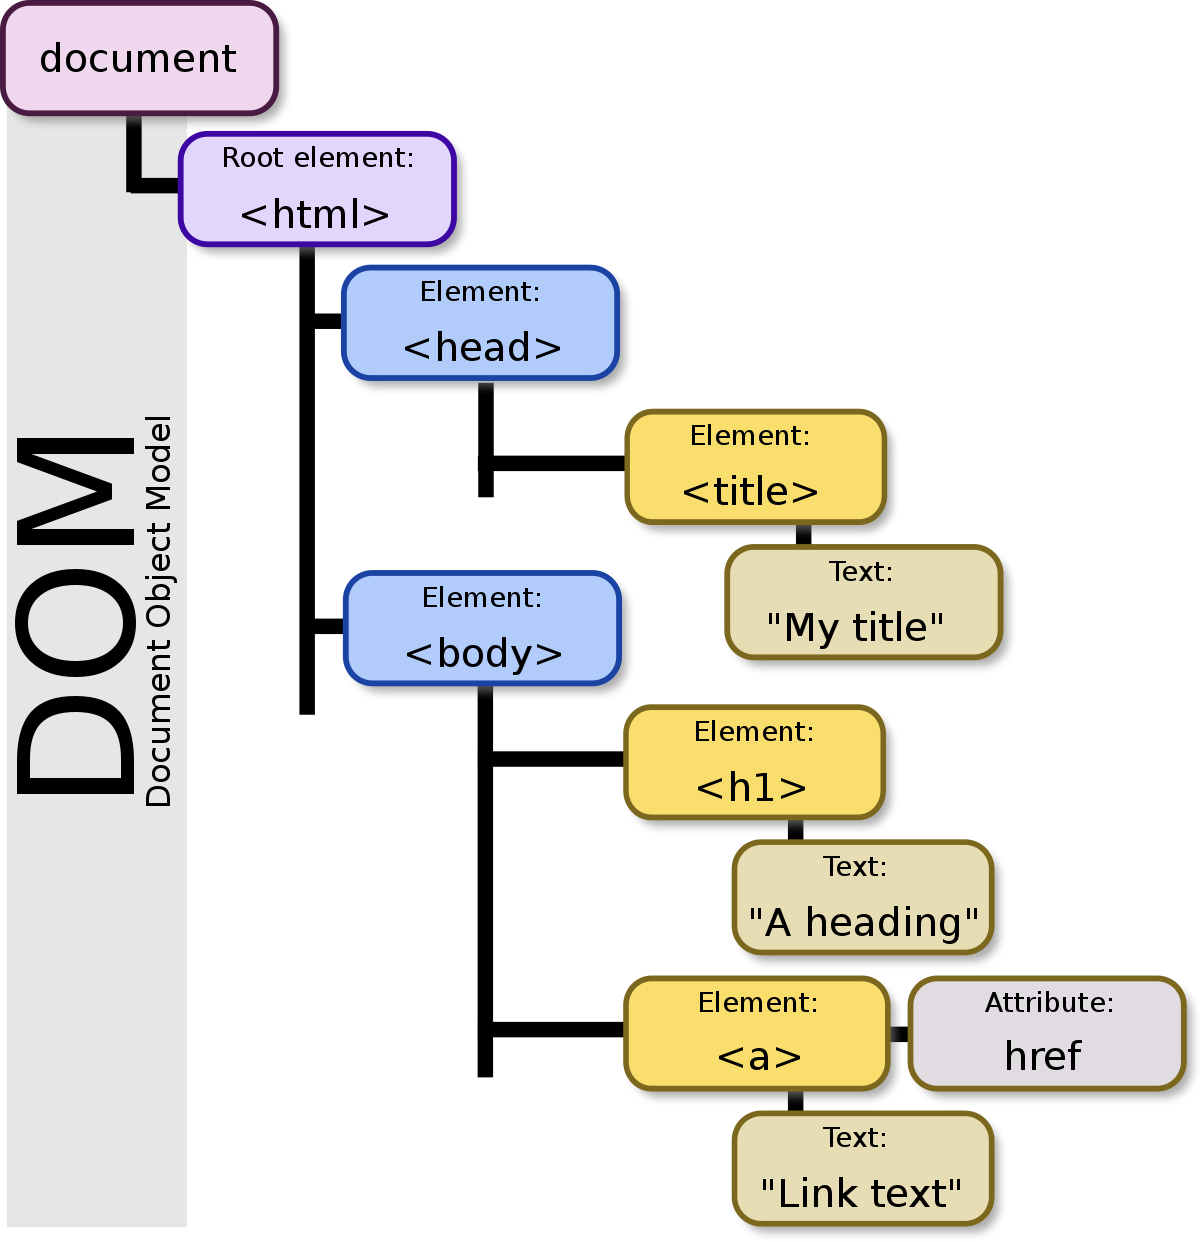
\includegraphics[width=0.8\textwidth]{figures/dom}
\label{fig:dom}
\caption{}
\end{figure}

\section{DOM as API}
\paragraph{} The DOM is a programming interface (API) for HTML. The DOM represents the page so that their structure, style, and content can be changed without needing to change or manipulate the source file(s) that define the page. This means that if we refresh a page, the result is a new instance of the page parsed into a new DOM, regardless of any changes that we'd made before the refresh. Note that this only holds if extra measures haven't been taken to persist any changes, for example, by using a cookie or browser local storage.
\paragraph{} The DOM operates in an Object-oriented way. Logical elements of the page are exposed to the user, who in this case is the programmer, as a containment hierarchy of objects which can, in turn, be modified.
\paragraph{} Be aware that many browsers extend the basic DOM to provide browser specific features but there is a common core that is shared across most modern browsers based upon the standards defined by the W3C and WHATWG.


\section{Accessing the DOM}
\paragraph{} Our browser’s JS environment gives us access to a global document object which we can access through the document object or else via the Window object, e.g. 

\begin{lstlisting}
	window.document
\end{lstlisting}

\paragraph{} Strictly we should access the document object and its contents as follows:

\begin{lstlisting}
	window.document. ...
\end{lstlisting}

\paragraph{} but both the window and document are exposed to JS as global objects so you might either approach both in real world code. As with most things, choose a style and be consistent in your own code, at least within any given project.
\paragraph{} It is a useful exercise to explore the document object in the browser console using the autocomplete function. Type in document and your browser should display a popup list of available attributes and functions that you can explore. This is a useful way to find out what is available on any given page.
\paragraph{} Once you access the DOM via the document object you can subsequently access, and explore, the document’s objects using the dot (“.”) operator.
\paragraph{} Try this out with some of your existing pages that you created earlier. Load one into a tab then open the browser console and explore which elements of your pages are exposed and available for manipulation. You should notice that, for example, the head and the body and the elements that they contain, and so on, are all accessible from JS. It is also worth noticing that what the DOM makes available to you is heavily dependent upon the contents of the specific page that you are on. A different page will likely have a very different DOM representation in terms of the detailed contents of the page, even if the broad structure, head and body, are the same. 
\paragraph{} Using the DOM, we can not only access but also modify, add, or remove elements so that we can change the contents of the current page, or even completely replace all of the HTML content with new content from code.



\section{Accessing Elements}
\paragraph{} One we have access to the DOM via the document or window.document objects we can access the elements within the page using the getElementById function, as we saw in previous examples:

\begin{lstlisting}
<!DOCTYPE html>
	<html> 
		<head>
			<title>SET08101 - Interacting with the DOM</title> 
		</head> 
	<body > 
		<p>
			<a href="#" onClick="addMessage();">Click Me</a>
		</p>
		<h1>OUTPUT:</h1>
		<p id="outputDemo"></p> 
		<script>
		function addMessage() { 
			document.getElementById("outputDemo").innerHTML = "HELLO NAPIER”
			}
		</script> 
	</body> 
</html> 
\end{lstlisting}

\paragraph{} In addition we can use other methods to retrieve elements of the DOM, especially if there isn't a specific ID to use. For example we have:

\begin{itemize}
\item getElementsByClassName()
\item getElementsByName()
\item getElementsByTagName()
\end{itemize}

\paragraph{} Which enable us to retrieve collections of elements that match either the specific class name attribute, name attribute, or tag name. Additionally there are also the querySelector() and querySelectorAll() methods which can be used, respectively, to access either the first element in the DOM that matches a given CSS selector or else all elements that match the supplied CSS selector.


\section{Adding \& Manipulating HTML DOM Elements}
\paragraph{} Just retrieving the contents of the page using the various get methods doesn't really help us much more than we could achieve if we just read the entire web page. So there are also mechanisms to let us manipulate the DOM by adding in new HTML elements, styling them with CSS, or attaching JS code to them. In the following example we create a new $<$h1$>$ element then create some text in a text node. We attach the text node to the $<$h1$>$ element by appending the text  node to it as a new child which causes the child text to effectively be enclosed in the parent $<$h1$>$ tags. The new heading tag and its child text are then appended to the document's body which causes the new heading to be displayed.

\begin{lstlisting}
<html>
  <head>
    <script>
       window.onload = function() {

         const heading = document.createElement("h1");
         const heading_text = document.createTextNode("DAKA DAKA");
         heading.appendChild(heading_text);
         document.body.appendChild(heading);
      }
    </script>
  </head>
  <body>
  </body>
</html>
\end{lstlisting}

\paragraph{} In addition to appending a child, all DOM elements let you manipulate them in a consistent way using the DOM element object API, for example using the various insert methods to place elements specifically in relation to existing elements instead of merely appending them. A summary of available methods for manipulating HTML DOM elements can be found in the W3Schools documentation\footnote{\url{https://www.w3schools.com/jsref/dom_obj_all.asp}}.

	

\section{Resources}
\paragraph{} There are many source of information about the Browser-based JS APIs: 
\begin{itemize}
\item The MDN JS Reference\footnote{\url{https://developer.mozilla.org/bm/docs/Web/JavaScript
}} not only includes reference information but also a set of tutorials for exploring JS
\item W3Schools JS and HTML DOM reference\footnote{\url{https://www.w3schools.com/jsref/}}
\item W3schools JS Tutorial\footnote{\url{https://www.w3schools.com/js/DEFAULT.asp}}
\end{itemize}


\section{Summary}
\paragraph{} In this chapter we've examined the JS APIs that most modern browsers support. Briefly we've considered:
\begin{itemize}
\item Looked at the role that JavaScript plays amongst other web technologies
\item Gained an understanding of the core JavaScript syntax
\item Discovered how JavaScript interacts with HTML, CSS, and the Browser
\end{itemize}

